\documentclass[CJKutf8,xcolor=pdftex,dvipsnames,table]{beamer}
\usepackage{hyperref}
\hypersetup{
  pdftitle={Signals and Systems},
  pdfauthor={Hong MingJian},
  pdfsubject={Introduction},
  pdfpagemode={FullScreen},
  colorlinks={true},
  linkcolor={blue},
}
\usepackage{CJKutf8}
\usepackage[export]{adjustbox}
\usepackage{mathptmx} %pdfTeX error: pdflatex (file fmex9.pfb): cannot open Type 1 font file for reading
                                                 %https://forum.ubuntu.com.cn/viewtopic.php?t=269943
\usepackage{mathtools}
\usepackage[mathscr]{urwchancal}

\usetheme{Madrid}%{Warsaw}
\usecolortheme{default}

%gets rid of bottom navigation bars
\setbeamertemplate{footline}[page number]{}
%gets rid of navigation symbols
\setbeamertemplate{navigation symbols}{}

\begin{document}
\begin{CJK*}{UTF8}{song}

  \title{\CJKfamily{hei} 数字信号处理}
  \subtitle{\CJKfamily{hei} 第5讲:连续时间傅立叶变换}
  \author{\CJKfamily{hei} 洪明坚}
  \institute{\CJKfamily{hei} 重庆大学软件学院}
  \date{\today}

  \AtBeginSection[]
  {
    \begin{frame}
      \frametitle{Outline}
      \tableofcontents[currentsection]
    \end{frame}
  }

  \frame{\titlepage}
  \frame{\frametitle{目录}\tableofcontents}
  
  \section{连续时间傅立叶变换}
  
  %% PAGE
  \begin{frame}
    \frametitle{傅立叶变换的引入}
    \begin{itemize}
    \item 周期为$T$的方波串 \\
	\begin{tabular}{ll}
	\raisebox{-.5\height}

    \begin{math}
x(t) = 
\left\{
    \begin {aligned}
         & 1 \quad & |t| < T_1 \\
         & 0 \quad & T_1 < |t| < T/2                  
    \end{aligned}
\right.
	\end{math}

&
    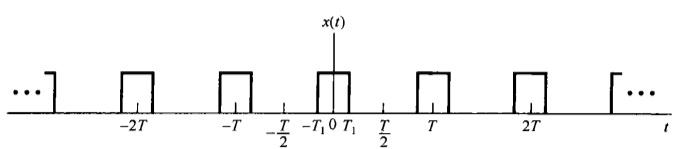
\includegraphics[valign=m,scale=.3]{ss-c-f4-1}    \\
    \end{tabular}  

  	\item 傅立叶级数的系数
   	\[ c_k = \frac{2sin(k\omega_0 T_1)}{k\omega_0 T}\] 
	可以写成
	\[
	Tc_k = \left. \frac{2sin(\omega T_1)}{\omega} \right\rvert_{\omega=k\omega_0}
	\]
	
    \end{itemize}      
  \end{frame}  

  %% PAGE
  \begin{frame}
    \frametitle{傅立叶变换的引入}
    \begin{itemize}
    \item $Tc_k$及其包络(envelop)曲线$\frac{2sin(\omega T_1)}{\omega}$的图像:(a)$T=4T_1$, (b)$T=8T_1$, (c)$T=16T_1$
		    \begin{center}
		   	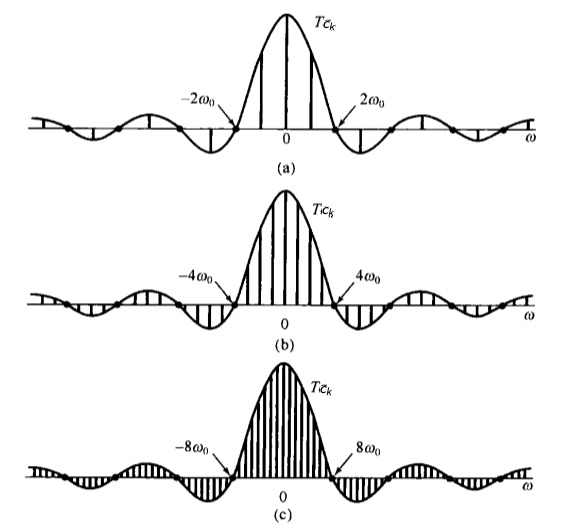
\includegraphics[scale=.27]{ss-c-f4-2}
    		\end{center}
	\item 固定$T_1$,随着$T$的增加,傅立叶系数是对包络曲线的越来越密集的采样。当$T \to \infty$时,一个非周期的方波函数的傅立叶系数趋近于该包络曲线。
    \end{itemize}

  \end{frame}    
   
  %% PAGE
  \begin{frame}
    \frametitle{傅立叶变换的定义}
    \begin{itemize}
    \item 对于任意函数$x(t)$,定义
    \begin{itemize}
    	\item 傅立叶变换
    	\[
			X(j\omega) = \int_{-\infty}^{\infty}x(t)e^{-j\omega t}dt    
    	\]
    	\item 傅立叶逆变换
    	\[
			x(t) = \frac{1}{2\pi}\int_{-\infty}^{\infty}X(j\omega)e^{j\omega t}d\omega    
    	\]    
    	\end{itemize}
    \end{itemize}

  \end{frame}     
   
  %% PAGE
  \begin{frame}
    \frametitle{傅立叶变换存在的充分条件}
    \begin{itemize}
    \item 能量条件
    \[
    	 \int_{-\infty}^{\infty}|x(t)|^2dt < \infty
    \]
    \item 波形条件
    \begin{itemize}
    	\item 绝对可积
    	\[
			\int_{-\infty}^{\infty}|x(t)|dt < \infty    
    	\]
    	\item 在任何有限区间内,只有有限个最大最小值
		\item 在任何有限区间内,只有有限个不连续点
   
    	\end{itemize}
    \end{itemize}

  \end{frame} 
     
  %% PAGE
  \begin{frame}
    \frametitle{例子}
    \begin{itemize}
    \item 指数函数
    \[
		x(t) = e^{at}u(t), a>0    
    \]
    \[
    	X(j\omega) = \int_{0}^{\infty}e^{-at}e^{-j\omega t}dt =\left. -\frac{1}{a+j\omega}e^{-(a+j\omega)t)} \right\rvert_{0}^{\infty} = \frac{1}{a+j\omega}
    \]
    
    	\begin{center}
      	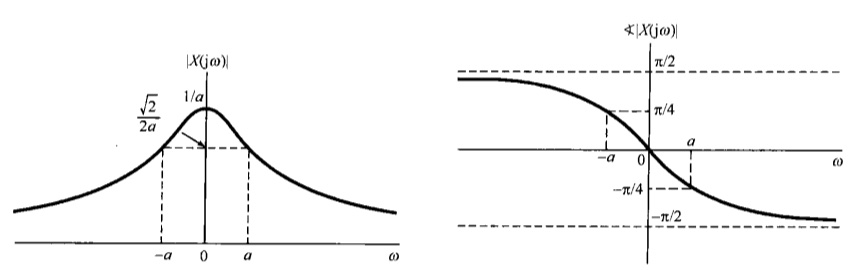
\includegraphics[scale=.37]{ss-c-f4-5}
    	\end{center}
    \end{itemize}

  \end{frame} 
     
  %% PAGE
  \begin{frame}
    \frametitle{例子}
    \begin{itemize}
    \item 高斯函数
    \[
		x(t) = e^{at^2}, a > 0    
    \]
    \[
    	X(j\omega) = \sqrt{\frac{\pi}{4}}e^{-\frac{\omega^2}{4a}}
    \]
    
    	\begin{center}
      	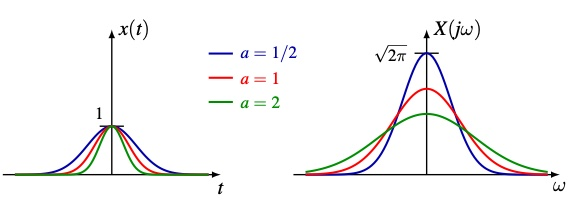
\includegraphics[scale=.5]{ftgaussian}
    	\end{center}
    \end{itemize}

  \end{frame} 
       
  %% PAGE
  \begin{frame}
    \frametitle{例子}
    \begin{itemize}
    \item 单位冲激函数$x(t) = \delta(t)$
    \[
    	X(j\omega) = \int_{-\infty}^{\infty}\delta(t)e^{-j\omega t}dt = 1
    \]
    逆变换
    \[
    	\delta(t) = \frac{1}{2\pi}\int_{-\infty}^{\infty}e^{j\omega t}d\omega
    \]
    \item DC信号$x(t)=1$    
    \[
    	X(j\omega) = \int_{-\infty}^{\infty}e^{-j\omega t}dt = \int_{-\infty}^{\infty}e^{j\omega t}dt = 2\pi\delta(\omega)
    \]
    逆变换
    \[
    	1 = \frac{1}{2\pi}\int_{-\infty}^{\infty}2\pi\delta(\omega)e^{j\omega t}d\omega
    \]
    \end{itemize}

  \end{frame} 

  %% PAGE
  \begin{frame}
    \frametitle{例子}
    \begin{itemize}    
    \item 复指数信号$x(t)=e^{j\omega_0 t}$
        \begin{align*}
 		X(j\omega) & = \int_{-\infty}^{\infty}e^{j\omega_0 t}e^{-j\omega t}dt \\
		& = \int_{-\infty}^{\infty}e^{j(\omega-\omega_0) t}dt    \\
		& = 2\pi\delta(\omega-\omega_0)
    	\end{align*} 
	逆变换
    \[
    	e^{j\omega_0 t} = \frac{1}{2\pi}\int_{-\infty}^{\infty}2\pi\delta(\omega-\omega_0)e^{j\omega t}d\omega
    \]

    \end{itemize}

  \end{frame}     
     
  %% PAGE
  \begin{frame}
    \frametitle{例子}
    \begin{itemize}
    \item 矩形脉冲函数
    \[
x(t) = 
\left\{
    \begin {aligned}
         & 1 \quad & |t| < T_1 \\
         & 0 \quad & otherwise                  
    \end{aligned}
\right.
	\]
	\[
		X(j\omega) = \int_{-T_1}^{T_1}e^{-j\omega t}dt = 2\frac{sin(\omega T_1)}{\omega}=2T_1sinc(\frac{\omega T_1}{\pi})
	\]
    
    	\begin{center}
      	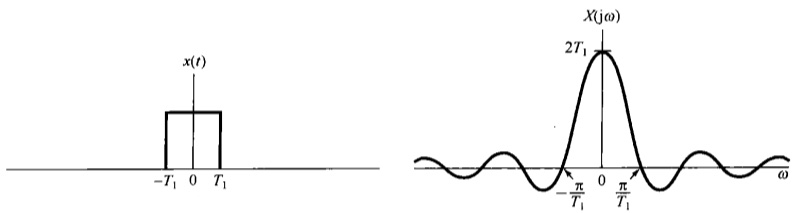
\includegraphics[scale=.37]{ss-c-f4-8}
    	\end{center}
	
		\begin{itemize}
		\item 其中
    	\[
    		sinc(\theta) = \frac{sin(\pi\theta)}{\pi\theta}
    	\]	
		\end{itemize}
    \end{itemize}

  \end{frame}      
     
  %% PAGE
  \begin{frame}
    \frametitle{例子}
    \begin{itemize}
    \item 反过来
    \[
X(j\omega) = 
\left\{
    \begin {aligned}
         & 1 \quad & |\omega| < W \\
         & 0 \quad & otherwise                  
    \end{aligned}
\right.
	\]
	\[
		x(t) = \frac{1}{2\pi}\int_{-W}^{W}e^{j\omega t}dt = \frac{sin(W t)}{\pi t} = \frac{W}{\pi}sinc(\frac{Wt}{\pi})
	\]
    
    	\begin{center}
      	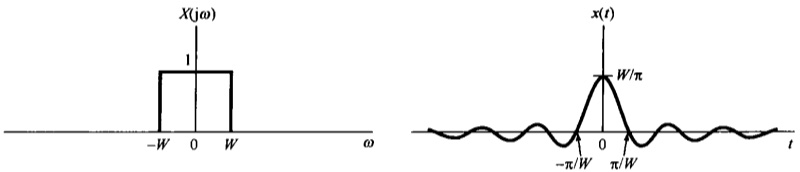
\includegraphics[scale=.37]{ss-c-f4-9}
    	\end{center}
	
		\begin{itemize}
		\item 其中
    	\[
    		sinc(\theta) = \frac{sin(\pi\theta)}{\pi\theta}
    	\]	
		\end{itemize}	
    \end{itemize}

  \end{frame} 
     
  %% PAGE
  \begin{frame}
    \frametitle{Questions}
    \begin{itemize}
    \item Any questions?
    \end{itemize}
    \begin{center}
      
\includegraphics[scale=.5]{question}
    \end{center}
  \end{frame} 
  
  \section{周期信号的傅立叶变换}
  
  %% PAGE
  \begin{frame}
    \frametitle{周期信号的傅立叶变换}
    \begin{itemize}
    \item 周期信号$x(t)$有傅立叶级数表示
    \[ 
    	x(t)=\sum_{k=-\infty}^{\infty}c_k e^{jk\omega_0 t} 
    \]
    \item 它的傅立叶变换
    	\begin{align*}
 		X(j\omega) & = \int_{-\infty}^{\infty}x(t)e^{-j\omega t}dt    \\
		& = \int_{-\infty}^{\infty}\sum_{k=-\infty}^{\infty}c_k e^{jk\omega_0 t}e^{-j\omega t}dt    \\
		& = \sum_{k=-\infty}^{\infty}c_k \int_{-\infty}^{\infty}e^{jk\omega_0 t}e^{-j\omega t}dt  \\
		& = \sum_{k=-\infty}^{\infty}2\pi c_k \delta(\omega-k\omega_0)
    	\end{align*}    
    \end{itemize}
  \end{frame}
  
  %% PAGE
  \begin{frame}
    \frametitle{例子:sin和cos}
    \begin{center}
      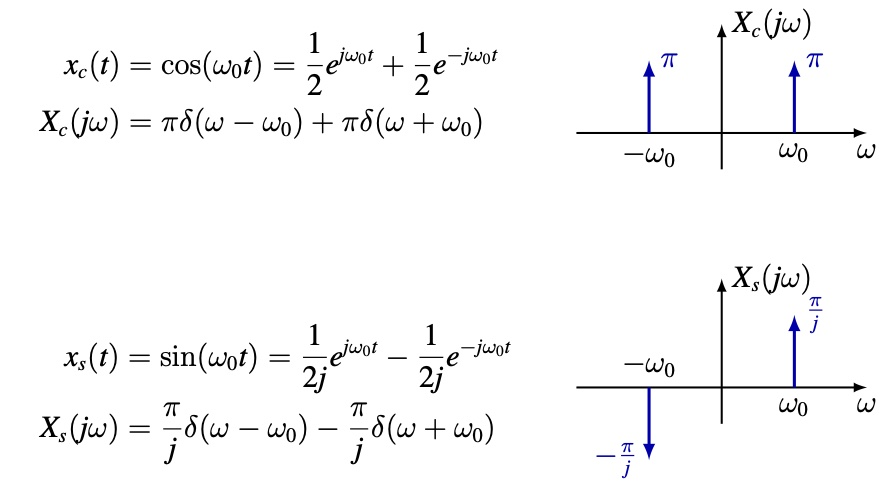
\includegraphics[scale=.4]{ftsincos}
    \end{center}    
  \end{frame}

  %% PAGE
  \begin{frame}
    \frametitle{例子:周期方波}
    \begin{center}
      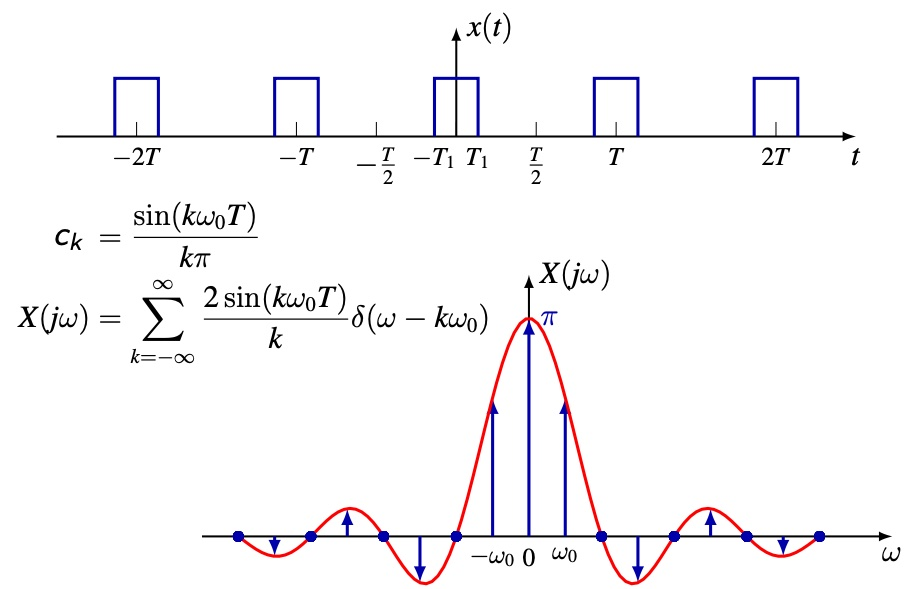
\includegraphics[scale=.35]{ftpsquare}
    \end{center}    
  \end{frame}    
    
  %% PAGE
  \begin{frame}
    \frametitle{例子:周期单位冲激串}
    \begin{center}
      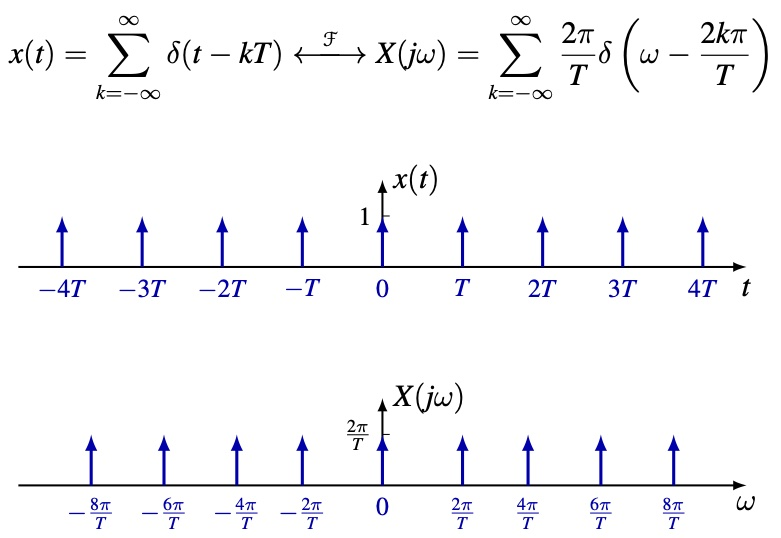
\includegraphics[scale=.35]{ftpimpulse}
    \end{center}    
  \end{frame}    
    
  %% PAGE
  \begin{frame}
    \frametitle{基本傅立叶变换对}
    \begin{center}
      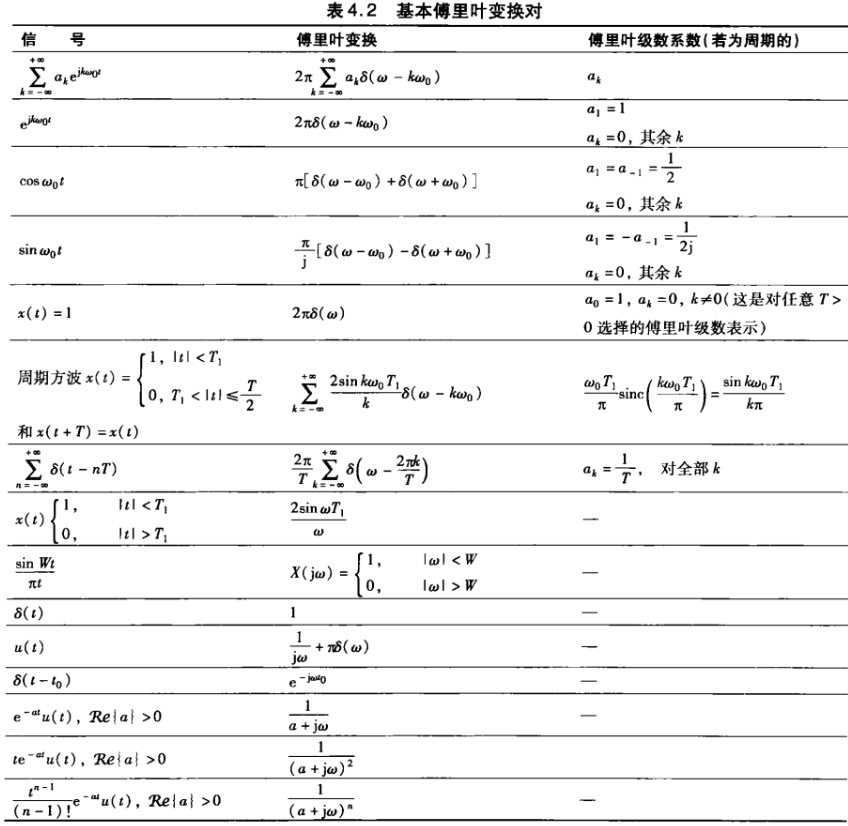
\includegraphics[scale=.29]{ss-c-t4-2}
    \end{center}
  \end{frame} 
    
  %% PAGE
  \begin{frame}
    \frametitle{Questions}
    \begin{itemize}
    \item Any questions?
    \end{itemize}
    \begin{center}
      
\includegraphics[scale=.5]{question}
    \end{center}
  \end{frame}   

	\section{连续时间傅立叶变换的性质}

  %% PAGE
  \begin{frame}
    \frametitle{性质}
    \begin{itemize}
    \item 线性:若$x(t) \xleftrightarrow{\mathscr{F}} X(j\omega)$, $y(t)\xleftrightarrow{\mathscr{F}}Y(j\omega)$,则
    \[
    ax(t)+by(t) \xleftrightarrow{\mathscr{F}} aX(j\omega)+bY(j\omega)
    \]
    \item 时移:$x(t-t_0) \xleftrightarrow{\mathscr{F}} e^{-j\omega t_0}X(j\omega)$
%    \item 共轭:$x^{*}(t) \xleftrightarrow{\mathscr{F}} X^{*}(-j\omega)$
    \item 微分:$\frac{dx(t)}{dt} \xleftrightarrow{\mathscr{F}} j\omega X(j\omega)$
%    \item 积分:$\int_{-\infty}^{t}x(\tau)d\tau \xleftrightarrow{\mathscr{F}} \frac{1}{j\omega} X(j\omega)+\pi X(0)\delta(\omega)$
%    \item 尺度变换:$x(at) \xleftrightarrow{\mathscr{F}} \frac{1}{|a|}X(\frac{j\omega}{a})$
	\end{itemize}
  \end{frame}    

  %% PAGE
  \begin{frame}
    \frametitle{性质}
    \begin{itemize}
    \item 对偶性(Duality)
    	\begin{itemize}
		\item
\begin{align*}
    \delta(t) & \xleftrightarrow{\mathscr{F}} 1  \\        
        1 & \xleftrightarrow{\mathscr{F}} 2\pi\delta(\omega) 
\end{align*}    
		\item
\begin{align*}
\delta(t-t_0) & \xleftrightarrow{\mathscr{F}} e^{-j\omega t_0} \\
e^{j\omega_0 t} & \xleftrightarrow{\mathscr{F}} 2\pi\delta(\omega-\omega_0) 
\end{align*}   

		\item    
    		\begin{center}
      		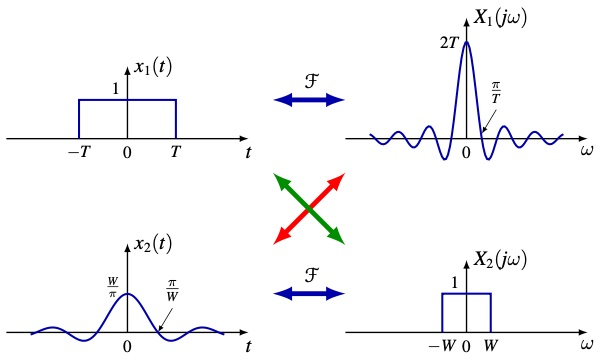
\includegraphics[scale=.3]{ftduality}
    		\end{center}
		\end{itemize}

%    \[
%x(t) = 
%\left\{
%    \begin {aligned}
%         & 1 \quad & |t| < T_1 \\
%         & 0 \quad & otherwise                  
%    \end{aligned}
%\right. \xleftrightarrow{\mathscr{F}} \frac{2sin(\omega T_1)}{\omega} \hspace{1cm}
%\frac{sin(Wt)}{\pi t} \xleftrightarrow{\mathscr{F}} 
%X(j\omega) = 
%\left\{
%    \begin {aligned}
%         & 1 \quad & |\omega| < W \\
%         & 0 \quad & otherwise                  
%    \end{aligned}
%\right. 
%    \]  
   
      
    \end{itemize}

  \end{frame}    

	
  %% PAGE
  \begin{frame}
    \frametitle{性质}
    \begin{itemize}
    \item 帕斯瓦尔定理
    \[
    \int_{-\infty}^{\infty}|x(t)|^2dt=\frac{1}{2\pi}\int_{-\infty}^{\infty}|X(j\omega)|^2d\omega
    \]
    \item 卷积定理:LTI系统的单位冲激响应$h(t)$,频率响应
    \[
    H(j\omega)=\mathscr{F}(h(t))=\int_{\mathbb{R}}h(t)e^{-j\omega t}dt
    \]
    则
    \[
    h(t)*x(t) \xleftrightarrow{\mathscr{F}} H(j\omega)X(j\omega)
    \]
    	
    \end{itemize}
  \end{frame}   
  	
  %% PAGE
  \begin{frame}
    \frametitle{例子}
    \begin{itemize}
    \item 理想低通滤波器 \\
	\begin{tabular}{ll}
	\raisebox{-.5\height}

    \begin{math}
H(j\omega) = 
\left\{
    \begin {aligned}
         & 1 \quad & |\omega| < \omega_c \\
         & 0 \quad & otherwise                  
    \end{aligned}
\right.
	\end{math}

&
    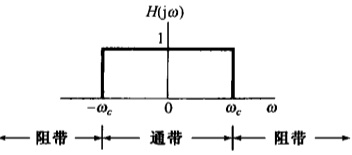
\includegraphics[valign=m,scale=.35]{ss-c-f4-20}    \\
    \end{tabular}      
    
    的单位冲激响应
    \[
    h(t)=\mathscr{F}^{-1}(H(j\omega))=\frac{sin(\omega_c t)}{\pi t}
    \]
    \begin{center}
      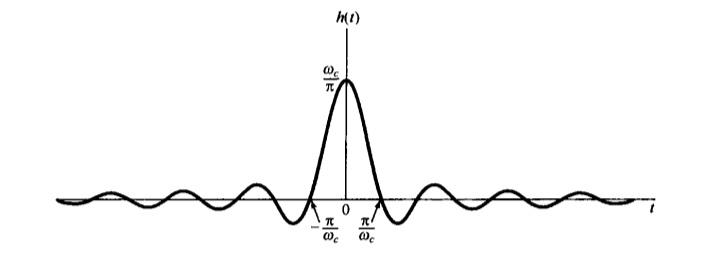
\includegraphics[scale=.4]{ss-c-f4-21}
    \end{center}
    因为$t<0$时$h(t)\neq 0$,所以该滤波器不是因果的
    
    \end{itemize}
  \end{frame}   

  %% PAGE
  \begin{frame}
    \frametitle{性质汇总}
    \begin{center}
      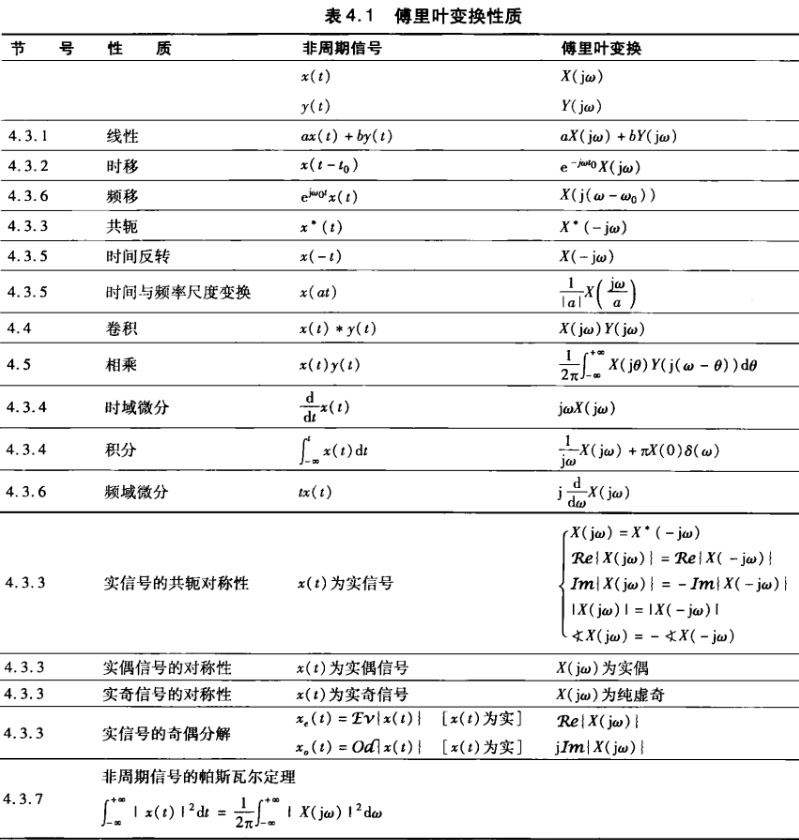
\includegraphics[scale=.28]{ss-c-t4-1}
    \end{center}
  \end{frame}  

  
  %% PAGE
  \begin{frame}
    \frametitle{Questions}
    \begin{itemize}
    \item Any questions?
    \end{itemize}
    \begin{center}
      
\includegraphics[scale=.5]{question}
    \end{center}
  \end{frame}  
        
\end{CJK*}
\end{document}

%%% Local Variables: 
%%% mode: latex
%%% TeX-master: t
%%% End: 
